%% ---------------------------------------------------------------------------------------------------------------------

\chapter{Introduction}\label{ch:introduction}

In today's modern society, software has become an integral part of many industries and areas of life.
The security of that software is very important, because successful attacks on it can have serious implications,
especially in the case of critical infrastructures like energy and food supply chains or medical services.
It is therefore important to try reducing the attack surface as best as possible.
In the last decade, there has been an ongoing adoption of memory-safe languages for many different applications.
Such languages include for example Google's Go, Rust, Nim, and even Java.
Memory safety is one of the most important areas of software security, because a large number of vulnerabilities is
caused by memory access bugs~\cite{heffley2004}.
In fact, Microsoft for example reports that memory safety accounts for around \checkNum{70\%} of all their
bugs~\footnote{\scriptsize\url{https://msrc-blog.microsoft.com/2019/07/16/a-proactive-approach-to-more-secure-code/}}.
To reduce the risk of such vulnerabilities, memory-safe languages provide different mechanisms to protect potentially
dangerous operations, such as accessing raw memory, dereferencing raw pointers, or arbitrary conversions between
incompatible types.
However, these languages often also provide ways for developers to explicitly circumvent the safety measures to various
degrees.

This thesis is focused on the Go programming language.
Go uses a strict typing system with limiting rules on pointer access and cast operations and automatic memory management
to achieve a high level of memory and thread safety~\cite{sibiryov2017}, but it also offers the \unsafe{} package.
This package is an \acrshort{API} built into the language that allows arbitrary access to raw pointers, similar to the
way pointers in C behave.
There are legitimate use cases for this, such as in an application with time and memory constraints that needs to cast
values to different types without reallocating them, or to access hardware when building a driver.

\begin{hero}[Thesis contribution big picture]
    The high-level objective of this thesis is to explore the Go \unsafe{} \acrshort{API}, both by finding possible
    security vulnerabilities and by analyzing how it is used in the wild.
\end{hero}

It is dangerous to use the \unsafe{} \acrshort{API} because when used incorrectly it can cause memory safety bugs that
lead to exploitable security vulnerabilities, as is shown in this thesis.
There can be buffer overflows leading to possible code injections when incompatible types with different sizes or
memory alignments are converted into each other, or the compiler may be unable to correctly determine the lifetime of
a value and allocate it on a function stack instead of the program heap, which can lead to \textit{use-after-free}i
vulnerabilities and with them all kinds of malicious program behaviors.
Thus, when \unsafe{} code is used it must be audited by the developers at least.
Furthermore, even after an initial code review it is important that security researchers can effectively analyze the
code base for potential misuses of \unsafe{} code, and administrators who deploy the software to their systems should
be aware of or analyze the possible consequences as well.

Checking \unsafe{} code in a project can however be hard because it can be introduced not only through first-party
code, but also through dependencies.
Recently, Evans et al.~\cite{evans2020} showed that in Rust programs \unsafe{} blocks are often introduced through
third-party libraries.
It might not be directly obvious which dependencies contain \unsafe{} code and should be audited, and checking all of
them is tedious and would create a tremendous cost in terms of development time.
Therefore, security analysts, developers, and administrators need tools that support them in identifying \unsafe{}
code usages in their project including its dependencies and assessing their risk.
There are suitable tools for other languages such as \toolCargoGeiger{} for Rust code, but previously there was no such
tool for Go.


%% ---------------------------------------------------------------------------------------------------------------------

\section{Problem Statement}\label{sec:introduction:problem-statement}

This section describes how the thesis objective is split into different parts that connect together.
Figure~\ref{fig:outline1} illustrates the organization and contributions of this thesis.

\begin{figure}[htp!]
    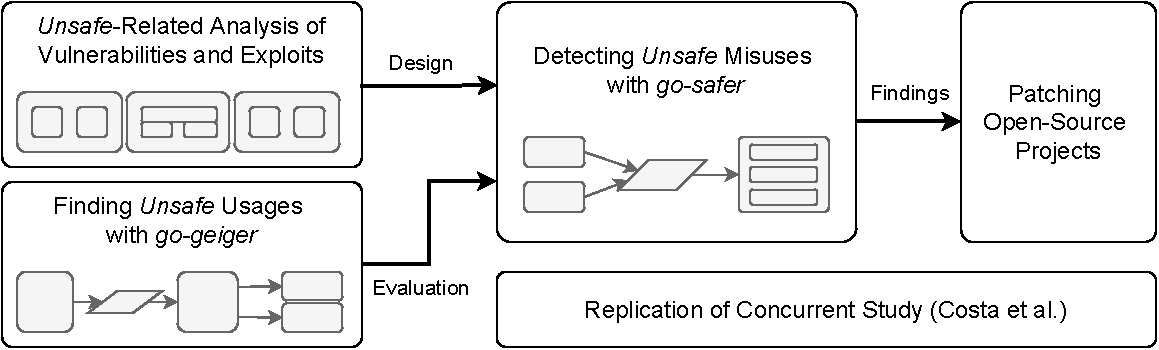
\includegraphics[width=\textwidth]{assets/figures/chapter1/outline1.pdf}
    \caption[Problem statement and thesis organization]
    {Problem statement and thesis organization.\newline\footnotesize~Parts in gray outline chapters and are shown in detail there.}
    \label{fig:outline1}
\end{figure}


\todo{replace Figure~\ref{fig:outline1} with a better, more organized representation of the thesis.}

First, a thorough manual analysis of possible vulnerabilities that can come from incorrect usages of the \unsafe{}
\acrshort{API}, including their consequences, is performed.
This is shown in the bottom left corner in the diagram.
Then, \toolGeiger{} is designed.
It is a novel tool that finds \unsafe{} usages in Go source code including its dependencies.
This tool is then used for an empirical study on the usage of \unsafe{} in the wild.
First, open-source Go projects are downloaded from \github{}.
They are then analyzed using \toolGeiger{}, which yields rawdata about \unsafe{} usages.
This data is then evaluated both quantitatively in terms of a statistical analysis, and qualitatively by sampling,
manually reviewing, and labeling code snippets from the identified \unsafe{} usages.
With these labels, insights are found about how and for what purpose the \unsafe{} \acrshort{API} is used.
This study, as well as \toolGeiger{}, is shown in the top row of the diagram.
Finally, to contribute to safer usage of \unsafe{}, a novel linter called \toolSafer{} is developed.
It is illustrated in the bottom center of Figure~\ref{fig:outline1}.
Its design is based on the \unsafe{}-related vulnerabilities and \unsafe{} usage patterns in open-source projects,
and it is evaluated using the labeled data set.

Thus, this thesis presents an analysis of vulnerabilities that are caused by misuses of the \unsafe{} \acrshort{API},
as well as two novel static analysis tools for Go developers.
It is worth noting that both tools have their own design, implementation, and evaluation sections in their respective
chapters, therefore this thesis does not use the typical standard outline.
%Furthermore, the methodology and results of the study on \unsafe{} code in open-source Go projects is presented in
%alongside the \toolGeiger{} tool, because first, the study data is gathered using \toolGeiger, and second, it
%simultaneously serves as an evaluation of \toolGeiger{}.


%% ---------------------------------------------------------------------------------------------------------------------

\section{Contributions}\label{sec:introduction:contributions}

The main contributions that are made in this thesis are the following:

\begin{enumerate}
    \item A thorough analysis of problems and consequences of usage patterns of the \unsafe{} \acrshort{API} in Go code
    with respect to a security context, revealing \checkNum{three} main areas of danger,

    \item \toolGeiger, a novel open-source static analysis tool to identify and count \unsafe{} usages in Go packages
    including their dependencies,

    \item a quantitative study of \unsafe{} code usage in \projsAnalyzed{} of the top \projsTotal{} most popular
    open-source Go projects on \github{},

    \item an in-depth study of \numberLabeledCodeSnippets{} code samples used in \projsForLabeledCodeSnippets{} selected
    projects, yielding a data set of two-dimensional manual classifications of usages and valuable insight into how and
    for what purpose unsafe code is used in Go applications,

    \item \toolSafer{}, a novel open-source, \toolVet{}-style, linter tool to find \checkNum{two} dangerous and common
    \unsafe{} usage patterns that were previously uncaught with existing tools, including an evaluation of its
    performance,

    \item the submission of \numberPRs{} pull requests to project maintainers with fixes to more than
    \numberBugsFixedRounded{} previously vulnerable code snippets in open-source Go libraries, and

    \item a replication of a related study on \unsafe{} Go code in concurrent work by Costa et al.~\cite{costa2020},
    including a comparison to this work and discussion of differences.
\end{enumerate}


%% ---------------------------------------------------------------------------------------------------------------------

\section{Outline}\label{sec:introduction:outline}

The remainder of this thesis is structured as described in the following: Chapter~\ref{ch:background} gives background
information on the Go \unsafe{} \acrshort{API} and other concepts needed for this thesis.
Chapter~\ref{ch:unsafe-security-problems} analyzes and discusses possible vulnerabilities caused by \unsafe{} code
usages.
Then, Chapter~\ref{ch:go-geiger} presents the design, implementation, and evaluation of \toolGeiger, the novel static
analysis tool which finds and counts \unsafe{} usages.
The chapter also describes the empirical study on \unsafe{} code in the wild, and presents the labeled data set of
\unsafe{} code samples.
After that, Chapter~\ref{ch:go-safer} shows the design, implementation, and evaluation of \toolSafer, the novel,
\unsafe{}-focused linter tool.
Next, Chapter~\ref{ch:related-work} discusses related and concurrent work.
Chapter~\ref{ch:discussion} discusses the meaning and impact of the findings and results of this work.
Threats to validity and possible future work are also presented there.
Finally, Chapter~\ref{ch:conclusion} concludes the work.
